\documentclass[table]{beamer}
%[]中可以使用draft、handout、screen、transparency、trancompress、compress等参数

%指定beamer的模式与主题
\mode<presentation>
{
  \usetheme{Madrid}
%\usetheme{Boadilla}
%\usecolortheme{default}
%\usecolortheme{orchid}
%\usecolortheme{whale}
%\usefonttheme{professionalfonts}
}

%\usetheme{Madrid}
%这里还可以选择别的主题:Bergen, Boadilla, Madrid, AnnArbor, CambridgeUS, Pittsburgh, Rochester, Warsaw, ...
%有导航栏的Antibes, JuanLesPins, Montpellier, ...
%有内容的Berkeley, PaloAlto, Goettingen, Marburg, Hannover, ...
%有最小导航栏的Berlin, Ilmenau, Dresden, Darmstadt, Frankfurt, Singapore, Szeged, ...
%有章和节表单的Copenhagen, Luebeck, Malmoe, Warsaw, ...

%\usecolortheme{default}
%设置内部颜色主题(这些主题一般改变block里的颜色);这个主题一般选择动物来命名
%这里还可以选择别的颜色主题,如默认的和有特别目的的颜色主题default,structure,sidebartab,全颜色主题albatross,beetle,crane,dove,fly,seagull,wolverine,beaver

%\usecolortheme{orchid}
%设置外部颜色主题(这些主题一般改变title里的颜色);这个主题一般选择植物来命名
%这里还可以选择别的颜色主题,如默认的和有特别目的的颜色主题lily,orchid,rose

%\usecolortheme{whale}
%设置字体主题;这个主题一般选择海洋动物来命名
%这里还可以选择别的颜色主题,如默认的和有特别目的的颜色主题whale,seahorse,dolphin

%\usefonttheme{professionalfonts}
%类似的还可以定义structurebold,structuresmallcapsserif,professionalfonts


% 控制 beamer 的风格,可以根据自己的爱好修改
%\usepackage{beamerthemesplit} %使用 split 风格
%\usepackage{beamerthemeshadow} %使用 shadow 风格
%\usepackage[width=2cm,dark,tab]{beamerthemesidebar}

%插入音标
\usepackage{tipa}
\AtBeginDocument{
  \renewcommand\textipa{\fontencoding{T3}\selectfont}
}
\AtBeginDocument{
  \renewcommand\textipa[2][r]{{\fontfamily{cm#1}\tipaencoding #2}}
}
\renewenvironment{IPA}[1][r]
 {\fontfamily{cm#1}\tipaencoding}
 {}

% 设定英文字体
%\usepackage{fontspec}
\usepackage[no-math]{fontspec}
\setmainfont{Times New Roman}
\setsansfont{Arial}
\setmonofont{Courier New}

% 设定中文字体
\usepackage[BoldFont,SlantFont,CJKchecksingle,CJKnumber]{xeCJK}
%\setCJKmainfont[BoldFont={Adobe Heiti Std},ItalicFont={Adobe Kaiti Std}]{Adobe Song Std}
\setCJKmainfont[BoldFont={Adobe Heiti Std},ItalicFont={Adobe Kaiti Std}]{WenQuanYi Micro Hei}
\setCJKsansfont{Adobe Heiti Std}
\setCJKmonofont{Adobe Fangsong Std}
\punctstyle{hangmobanjiao}

\defaultfontfeatures{Mapping=tex-text}
\usepackage{xunicode}
\usepackage{xltxtra}

\XeTeXlinebreaklocale "zh"
\XeTeXlinebreakskip = 0pt plus 1pt minus 0.1pt

\usepackage{setspace}
\usepackage{colortbl,xcolor}
\usepackage{hyperref}
%\hypersetup{xetex,bookmarksnumbered=true,bookmarksopen=true,pdfborder=1,breaklinks,colorlinks,linkcolor=blue,filecolor=black,urlcolor=cyan,citecolor=green}
\hypersetup{xetex,bookmarksnumbered=true,bookmarksopen=true,pdfborder=1,breaklinks,colorlinks,linkcolor=cyan,filecolor=black,urlcolor=blue,citecolor=green}

% 插入图片
\usepackage{graphicx}
\graphicspath{{figures/}}
% 图文混排
\usepackage{picins}
\usepackage{floatflt}

% 可能用到的包
\usepackage{amsmath,amssymb}
%插入多媒体
%\usepackage{media9}
%\usepackage{movie15}
\usepackage{multimedia}
\usepackage{multicol}
\usepackage{multirow}

% 定义一些自选的模板,包括背景、图标、导航条和页脚等,修改要慎重
% 设置背景渐变由10%的红变成10%的结构颜色
%\beamertemplateshadingbackground{red!10}{structure!10}
%\beamertemplatesolidbackgroundcolor{white!90!blue}
% 使所有隐藏的文本完全透明、动态,而且动态的范围很小
\beamertemplatetransparentcovereddynamic
% 使itemize环境中变成小球,这是一种视觉效果
\beamertemplateballitem
% 为所有已编号的部分设置一个章节目录,并且编号显示成小球
\beamertemplatenumberedballsectiontoc
% 将每一页的要素的要素名设成加粗字体
\beamertemplateboldpartpage

% item逐步显示时,使已经出现的item、正在显示的item、将要出现的item呈现不同颜色
\def\hilite<#1>{
 \temporal<#1>{\color{gray}}{\color{blue}}
    {\color{blue!25}}
}

\renewcommand{\today}{\number\year 年 \number\month 月 \number\day 日}

%五角星
\usepackage{MnSymbol}

%去除图表标题中的figure等
\usepackage{caption}
\captionsetup{labelformat=empty,labelsep=none}

\usepackage{tabu}
\usepackage{multirow}
%表格自动换行
\usepackage{tabularx} 

% 千分号
%\usepackage{textcomp}

%罗马数字
\makeatletter
\newcommand{\rmnum}[1]{\romannumeral #1}
\newcommand{\Rmnum}[1]{\expandafter\@slowromancap\romannumeral #1@}
\makeatother

%分栏
\usepackage{multicol}

%\usepackage{enumitem}
%\usepackage{enumerate}

%键盘
\usepackage{keystroke}

%插入源代码
\usepackage{listings}
\lstset{
  language=bash,                  % 程序语言名称:TeX, Perl, R, sh, bash, Awk
  basicstyle=\normalsize\tt,      %\tt指monospace字体族,程序源代码使用此族字体表示更加美观
  numbers=left,                   % 行号位置(左侧)
  numberstyle=\small,             % 行号字体的字号
  stepnumber=1,                   % 行号的显示步长
  numbersep=5pt,                  % 行号与代码间距
  backgroundcolor=\color{white},  % 背景色;需要 \usepackage{color}
  showspaces=false,               % 不显示空格
  showstringspaces=false,         % 不显示代码字符串中的空格标记
  showtabs=false,                 % 不显示 TAB
  tabsize=4, 
  frame=shadowbox,                % 把代码用带有阴影的框圈起来
  captionpos=b,                   % 标题位置
  breaklines=true,                % 对过长的代码自动断行
  breakatwhitespace=false,        % 断行只在空格处
  extendedchars=false,            % 解决代码跨页时,章节标题,页眉等汉字不显示的问题
  %escapeinside={\%*}{*},         % 跳脱字符,添加注释,暂时离开 listings 
  %escapeinside=``,
  commentstyle=\color{red!50!green!50!blue!50}\tt,  %浅灰色的注释
  rulesepcolor=\color{red!20!green!20!blue!20},     %代码块边框为淡青色
  keywordstyle=\color{blue!70}\bfseries\tt,         %代码关键字的颜色为蓝色,粗体
  identifierstyle=\tt,
  stringstyle=\tt,                % 代码字符串的特殊格式
  keepspaces=true,
  breakindent=1em,
  %breakindent=22pt,
  %breakindent=4em,
  breakautoindent=true,
  flexiblecolumns=true,
  aboveskip=1em,                  %代码块边框
  xleftmargin=2em,
  xrightmargin=2em
}

%\setbeamercolor{alerted text}{fg=magenta}
\setbeamercolor{bgcolor}{fg=yellow,bg=cyan}
%\setbeamercolor{itemize/enumerate body}{fg=green}

\begin{document}

%\includeonlyframes{current}

\logo{
\includegraphics[height=0.08\textwidth]{tijmu.png}}

% 在每个Section前都会加入的Frame
\AtBeginSection[]
{
  \begin{frame}<beamer>
    %\frametitle{Outline}
    \frametitle{教学提纲}
    \setcounter{tocdepth}{3}
    \begin{multicols}{2}
      \tableofcontents[currentsection,currentsubsection]
      %\tableofcontents[currentsection]
    \end{multicols}
  \end{frame}
}
% 在每个Subsection前都会加入的Frame
\AtBeginSubsection[]
{
  \begin{frame}<beamer>
%%\begin{frame}<handout:0>
%% handout:0 表示只在手稿中出现
    \frametitle{教学提纲}
    \setcounter{tocdepth}{3}
    \begin{multicols}{2}
    \tableofcontents[currentsection,currentsubsection]
    \end{multicols}
%% 显示在目录中加亮的当前章节
  \end{frame}
}

% 为当前幻灯片设置背景
%{
%\usebackgroundtemplate{
%\vbox to \paperheight{\vfil\hbox to
%\paperwidth{\hfil
\includegraphics[width=2in]{tijmu_charcoal.png}\hfil}\vfil}
%}
\begin{frame}[plain]
  \begin{center}
    {\Huge Linux系统概论\\}
    \vspace{1cm}
    {\LARGE 天津医科大学\\}
    %\vspace{0.2cm}
    {\LARGE 生物医学工程与技术学院\\}
    \vspace{1cm}
    {\large 2017-2018学年下学期(春)\\ 2016级生信班}
  \end{center}
\end{frame}
%}



%\includeonlyframes{current}

\title[Vim]{第七章\quad Vim编辑器}
\author[Yixf]{伊现富(Yi Xianfu)}
\institute[TIJMU]{天津医科大学(TIJMU)\\ 生物医学工程与技术学院}
\date{2018年6月}


\begin{frame}
  \titlepage
\end{frame}

\begin{frame}[plain,label=current]
  \frametitle{教学提纲}
  \setcounter{tocdepth}{3}
  \begin{multicols}{2}
    \tableofcontents
  \end{multicols}
\end{frame}


\section{引言}
\begin{frame}
  \frametitle{引言 | 纯文本 vs. 格式化文本}
  \begin{center}
    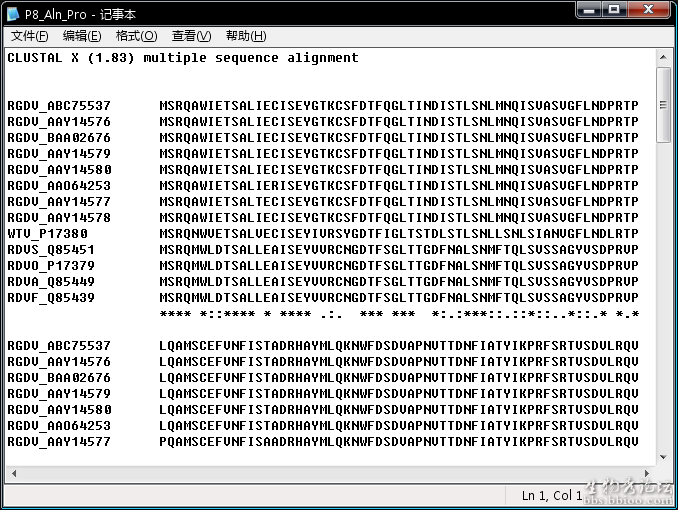
\includegraphics[width=5.9cm,height=6.45cm]{c7_txt.png}
    \vspace*{0.1cm}
    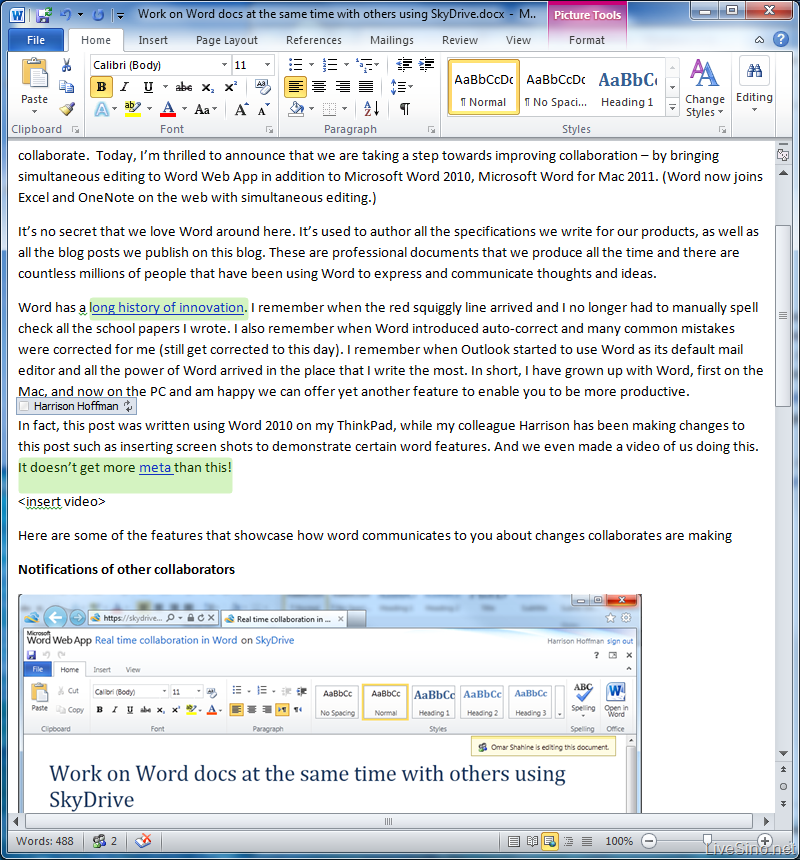
\includegraphics[width=6cm]{c7_word.png}
  \end{center}
\end{frame}

\begin{frame}
  \frametitle{引言 | 文本编辑器}
  \begin{center}
    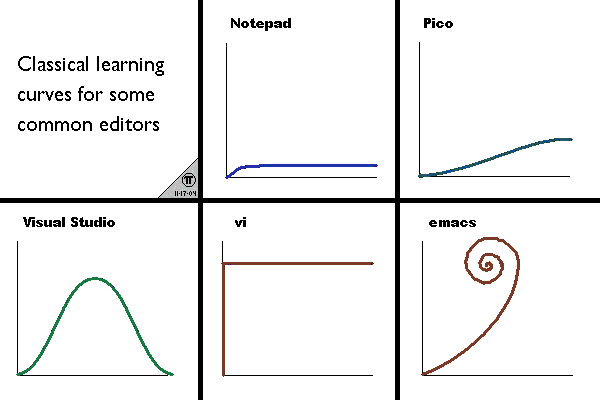
\includegraphics[width=10cm]{c7_editors_01.png}
  \end{center}
\end{frame}

\begin{frame}
  \frametitle{引言 | 文本编辑器}
  \begin{center}
    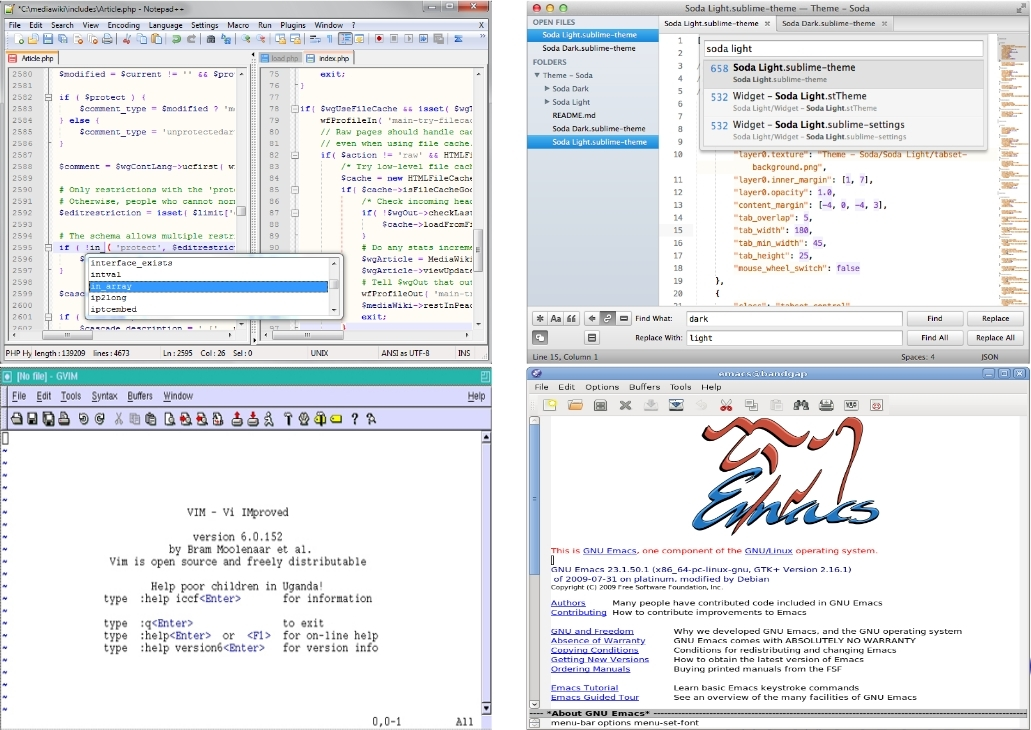
\includegraphics[width=11cm]{c7_editors_02.png}
  \end{center}
\end{frame}

\begin{frame}
  \frametitle{引言 | 文本编辑器}
  \begin{center}
    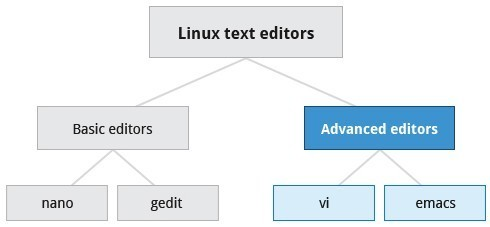
\includegraphics[width=11cm]{c7_editor_linux_01.jpg}
  \end{center}
\end{frame}

\begin{frame}
  \frametitle{引言 | 文本编辑器}
  \begin{block}{三类编辑器}
    Vim\qquad Emacs\qquad 其他
  \end{block}
  \pause
  \begin{block}{大腕版文本编辑器}
  \textit{“周围同事不是用Vi就是Emacs,你要是用UltraEdit,你都不好意思跟人家打招呼……什么插件呀、语法高亮呀、拼写检查呀、能给它开的都给它开着,就是一个字儿:酷!你说这么牛X一东西,怎么着学会也得小半年吧。半年!入门都远着呢,能学会移动光标就不错了,你还别说耗不起,就这还只是左右移动!!” }
  \begin{flushright}
    ——《大腕\textbullet 文本编辑器》
  \end{flushright}
\end{block}
\end{frame}

\begin{frame}
  \frametitle{引言 | 文本编辑器 | 学习经历}
  \begin{center}
    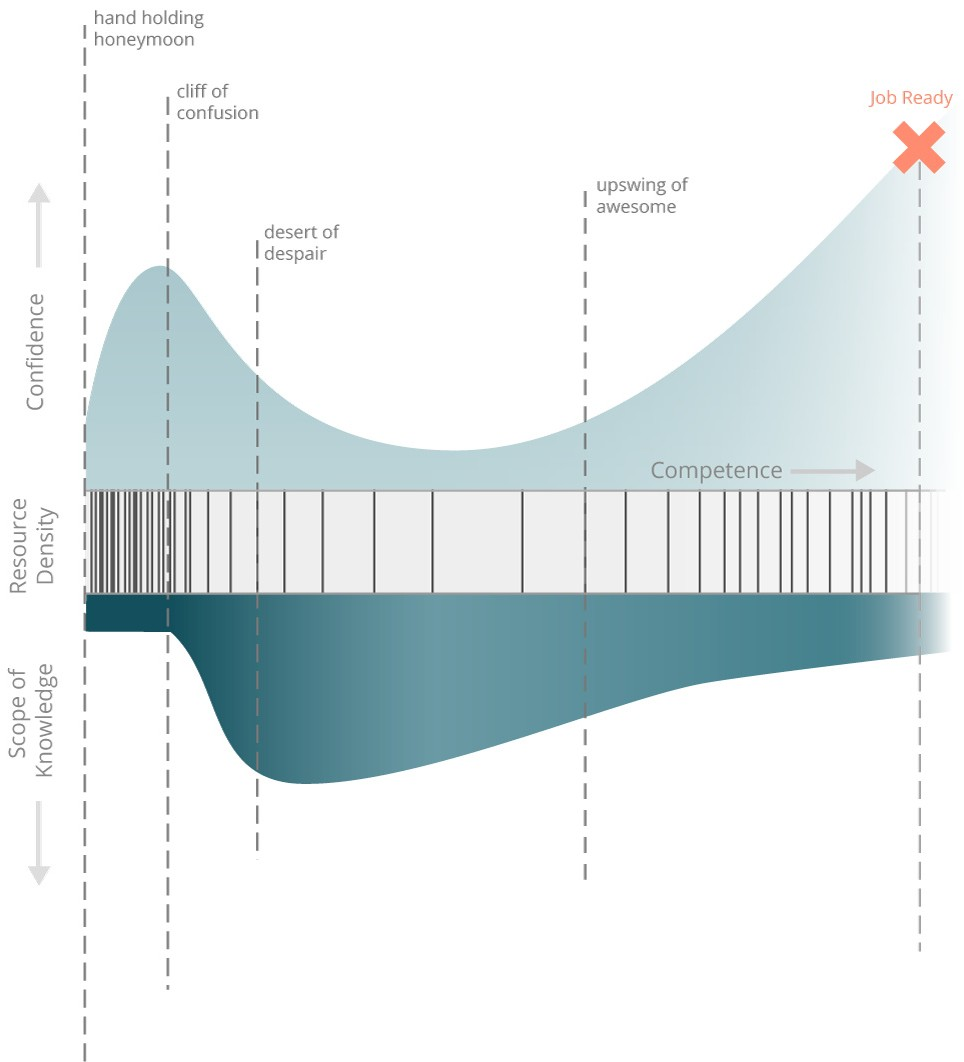
\includegraphics[width=11cm,height=9cm]{c7_learn_code.jpg}
  \end{center}
\end{frame}

\begin{frame}
  \frametitle{引言 | 文本编辑器 | 键盘磨损$\Rightarrow$用户习惯}
  \vspace{-0.5em}
  \begin{columns}
    \column{0.55\textwidth}
  \begin{block}{键盘磨损}
    \begin{itemize}
      \item W
      \item F5
      \item W、A、S、D
      \item W、A、S、D、U、I、J、K
      \item ALT+S或CTRL+ENTER
      \item CTRL+C和CTRL+V
      \item A+SHIFT+CTRL+1+2+3+4+……
      \item CTRL+ALT+DEL
      \item 小键盘
      \item 以D和回车为圆心的两个圆形
      \item ESC、H、J、K、L
      \item Ctrl+Alt+Shift
      \item ……
    \end{itemize}
   \end{block}
   \pause
    \column{0.05\textwidth}
    \column{0.4\textwidth}
   \begin{block}{用户习惯/职业}
    \begin{itemize}
      \item FIFA高手
      \item 论坛版主
      \item 游戏迷(CS,35*,…)
      \item 拳皇迷
      \item QQ狂人
      \item 网站编辑/转帖狂人
      \item 星际争霸迷
      \item 电脑白痴/该换电脑了
      \item 会计师/银行出纳
      \item “气管炎”
      \item Vim
      \item Emacs
      \item ……
    \end{itemize}
   \end{block}
 \end{columns}
\end{frame}

\section{Vim简介}
\begin{frame}
  \frametitle{Vim简介}
  Vim/vi是一个功能强大的全屏幕文本编辑器,是Linux/UNIX上最常用的文本编辑器,它的作用是创建、编辑、显示文本文件。Vim/vi没有菜单,只有命令。
\end{frame}

\subsection{vi版本}
\begin{frame}
  \frametitle{简介 | vi版本}
  %\begin{description}[<+-|alert@+>]
  \begin{description}[<+->]
    \item[vi] 由美国计算机科学家比尔·乔伊(Bill Joy)于1976年编写、并以BSD授权发布的文本编辑器。vi是“Visual”的不正规的缩写,来源于另外一个文本编辑器ex的命令visual。
    \item[Vim] Vi IMproved,从vi发展出来的一个文本编辑器,和Emacs并列成为类Unix系统用户最喜欢的编辑器。布莱姆·米勒在1991年发布第一个版本,现在是在开放源代码方式下发行的自由软件。Vim是Linux系统中最常用的vi版本,具有vi的所有特性,并添加了一些重要的改进,包括语法高亮、代码折叠和多级撤销等。 
    \item[Vile] Vi Like Emacs。试图将vi和Emacs的优点结合在一起。 
    \item[Vigor] 含有Vigor助手的vi,对抗Microsoft Office的Clippy。
    \item[Elvis] vi的升级版本,具有一些额外的特性。 
    \item[Nvi] vi的BSD版本。 
  \end{description}
\end{frame}

\subsection{学习Vim}
\begin{frame}[fragile]
  \frametitle{简介 | 学习}
  \begin{block}{\alert{入门学习}}
    %\begin{description}[<+-|alert@+>]
    \begin{description}[<+->]
      \item[Vim初学者教学] 在Linux系统\textcolor{red}{命令行下}输入:\verb|vimtutor|
      \item[Vim用户手册] 在 \textcolor{red}{Vim中}输入:\verb|:help user-manual@cn|(中文版),\verb|:help user-manual|(英文版)
      \item[Vim帮助系统] 在 \textcolor{red}{Vim中}输入:\verb|:help|
    \end{description}
  \end{block}
  {\footnotesize
  对于大多数用户来说,Vim有着一个比较陡峭的学习曲线。这意味着开始学习的时候可能会进展缓慢,但是一旦掌握一些基本操作之后,能大幅度提高编辑效率。\\
  为了帮助学习,Vim为初学者准备了Vim教学。通常可以在Linux系统命令行下输入“vimtutor”或者点击Windows系统桌面上的Vim教学图标进入。\\
  在Vim用户手册中更加详细得描述了Vim的基础和进阶功能。可以在Vim中输入“:help user-manual”进入用户手册。手册除了原始的英文版本之外,也被志愿者翻译成了各国文字,其中包括中文。\\
  新用户也应该学习Vim的帮助系统,可以在Vim中输入不带参数的“:help”来阅读主帮助文件。}
\end{frame}

\subsection{启动Vim}
\begin{frame}
  \frametitle{简介 | 启动 | \alert{方法}}
  \begin{table}
    \centering
    \rowcolors[]{1}{blue!20}{blue!10}
    \begin{tabularx}{\textwidth}{cXX}
      \hline
      \rowcolor{blue!50}命令 & 说明 & 结果\\
      \hline
      vim & 不使用文件名参数启动Vim & 启动一个空的Vim面板。退出前必须把所做的编辑保存到新文件中\\
      vim filename & 使用已有文件名作为参数 & 在Vim中打开已有的文件。保存时将更新文件中修改过的内容\\
      vim filename & 使用新文件名作为参数 & 保存时将使用指定的文件名创建新文件\\
      vim -R filename & 以只读模式打开文件 & 文件是只读的,不能保存修改(\alert{练习使用Vim命令的好方法})\\
      view filename & 同vim -R filename & ---\\
      vim -r filename & 以修复模式打开文件 & ---\\
      \hline
    \end{tabularx}
  \end{table}
\end{frame}

\begin{frame}
  \frametitle{简介 | 启动 | 界面}
  \begin{figure}
    \centering
    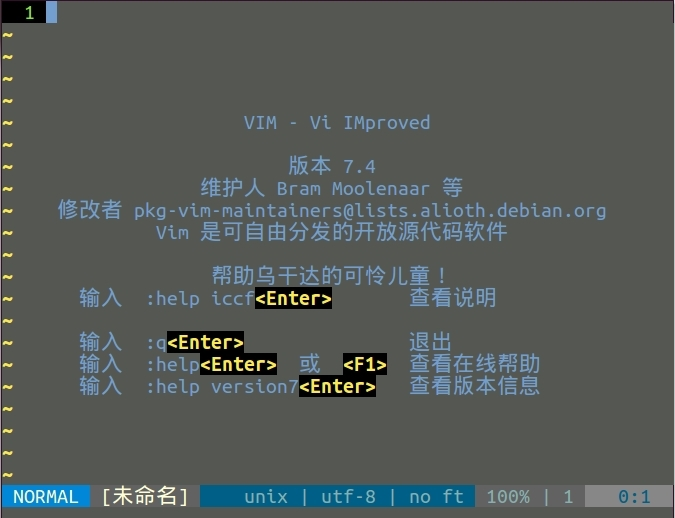
\includegraphics[width=5.8cm]{c7_vim_start_01.png}\quad
    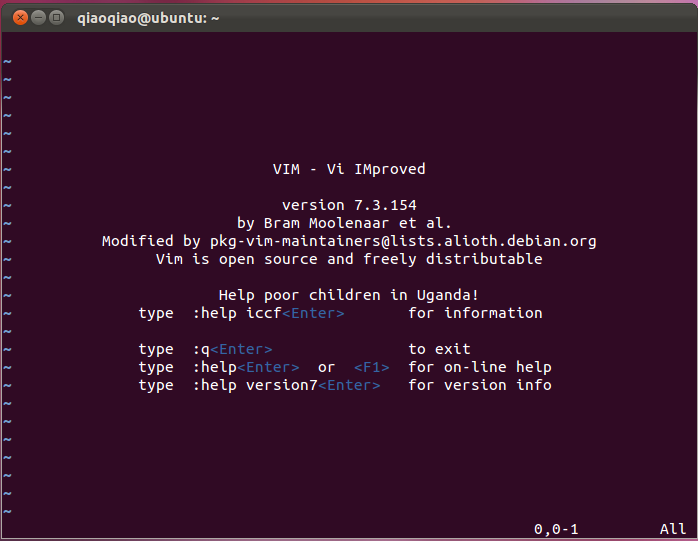
\includegraphics[width=5.8cm]{c7_vim_start_02.png}\\
    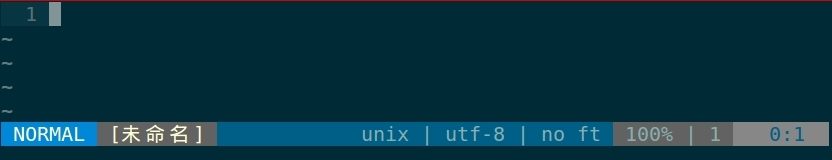
\includegraphics[width=12cm]{c7_vim_start_03.png}
  \end{figure}
\end{frame}

\begin{frame}[fragile]
  \frametitle{简介 | 启动 | 说明}
  %\begin{itemize}[<+-|alert@+>]
  \begin{itemize}[<+->]
    \item 行首的颚化符号(~)表示未使用的行。不以~开始却仍然是空白的,说明存在空格、制表符或其他不可见字符。
    \item 屏幕底部是状态行,显示文件名和光标所在的行等信息。
    \item 打开文件时,拒绝访问或显示只读,可能存在权限问题。
    \item 打开非文本文件可能会显示乱码,输入 \verb|:q!|直接退出即可。
    \item 启动Vim后默认进入命令模式。要输入文本,必须进入输入模式。
  \end{itemize}
\end{frame}

\subsection{状态行}
\begin{frame}
  \frametitle{简介 | 状态行}
  \begin{figure}
    \centering
    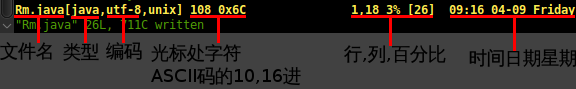
\includegraphics[width=12cm]{c7_vim_statusline_04.png}
    \vspace{0.2cm}
    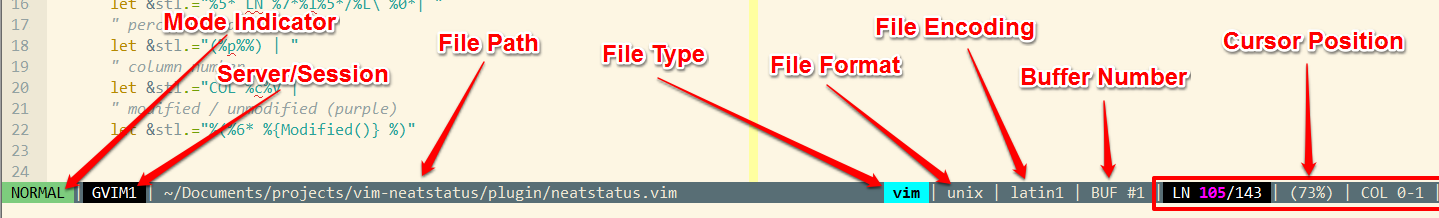
\includegraphics[width=12cm]{c7_vim_statusline_01.png}
    \vspace{0.2cm}
    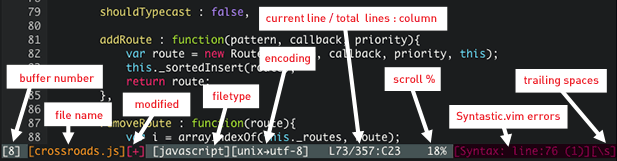
\includegraphics[width=12cm]{c7_vim_statusline_02.png}
  \end{figure}
\end{frame}

\subsection{工作模式}
\begin{frame}
  \frametitle{简介 | 工作模式 | \alert{主要模式}}
  %\begin{description}[<+-|alert@+>]
  \begin{description}[<+->]
    \item[命令模式(Command Mode)] Vim启动后的默认模式,所输入的任何内容都被解释成命令。在此模式中,用户可以执行一般的编辑器命令,比如移动光标、删除文本等等。在命令模式中,有很多方法可以进入输入模式,比较普通的方式是按“a”(append,追加)键或者“i”(insert,插入)键。
    \item[输入模式(Insert Mode)] 在此模式中,大多数按键都会向文本缓冲中插入文本,可以按ESC键回到命令模式。
    \item[末行模式(Last Line Mode)] 在末行模式中可以输入会被解释并执行的文本。例如执行命令(“:”键),搜索(“/”和“?”键)或者过滤命令(“!”键)。在命令执行之后,Vim返回到末行模式之前的模式,通常是普通模式(命令模式)。
  \end{description}
\end{frame}

\begin{frame}
  \frametitle{简介 | 工作模式 | 其他模式}
  %\begin{description}[<+-|alert@+>]
  \begin{description}[<+->]
    \item[可视模式] 与命令模式比较相似,但是移动命令会扩大高亮的文本区域。高亮区域可以是字符、行或者是一块文本。当执行一个非移动命令时,命令会被执行到这块高亮的区域上。
    \item[替换模式] 一个特殊的插入模式,在这个模式中可以做和插入模式一样的操作,但是每个输入的字符都会覆盖文本缓冲中已经存在的字符。在命令模式下按“R”键进入。
    \item[选择模式] 和无模式编辑器的行为比较相似。这个模式中,可以用鼠标或者光标键高亮选择文本,不过输入任何字符的话,Vim会用这个字符替换选择的高亮文本块,并且自动进入输入模式。
    \item[Ex模式] 和命令行模式比较相似,在使用“:visual”命令离开Ex模式前,可以一次执行多条命令。在命令模式下按“Q”键进入。
  \end{description}
\end{frame}

\begin{frame}
  \frametitle{简介 | 工作模式 | \alert{模式转换}}
  \begin{figure}
    \centering
    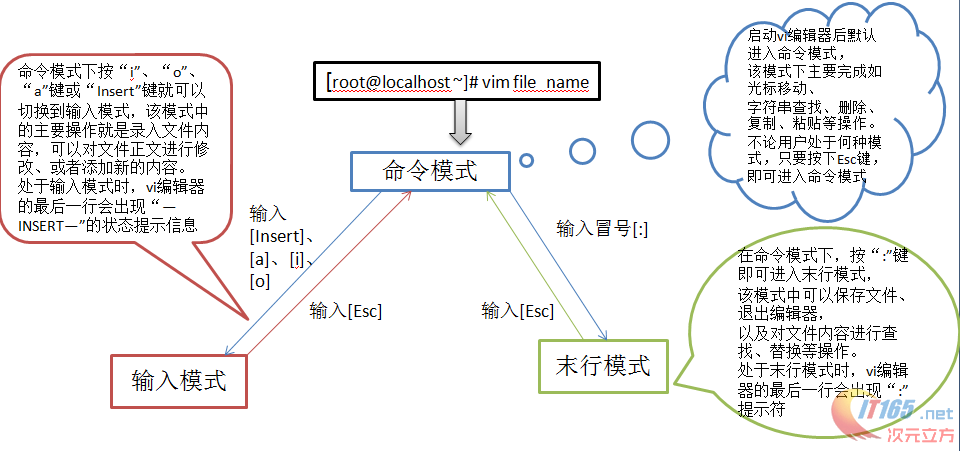
\includegraphics[width=12cm]{c7_vim_mode_01.png}
  \end{figure}
\end{frame}

\begin{frame}
  \frametitle{简介 | 工作模式 | 模式转换}
  \begin{figure}
    \centering
    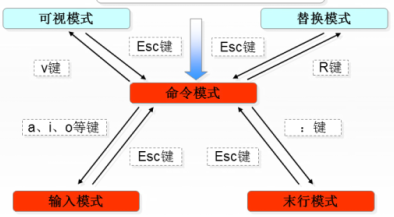
\includegraphics[width=10cm]{c7_vim_mode_07.png}
  \end{figure}
\end{frame}

\begin{frame}
  \frametitle{简介 | 工作模式 | 补充说明}
  %\begin{itemize}[<+-|alert@+>]
  \begin{itemize}[<+->]
    \item 注意状态栏中显示的工作模式及只读指示。
    \item 一般按Esc键即可退出其他模式。
    \item 可以按两次Esc键以确保回到命令模式。
    \item Vim命令区分大小写。
    \item 接下来介绍的命令绝大多数都基于命令模式。
  \end{itemize}
\end{frame}

\section{移动和定位}
\begin{frame}
  \frametitle{移动和定位 | \alert{基本移动}}
  \begin{figure}
    \centering
    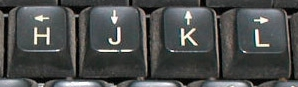
\includegraphics[width=5cm]{c7_vim_hjkl_01.jpg}
  \end{figure}
  \begin{table}
    \centering
    \rowcolors[]{1}{blue!20}{blue!10}
    \begin{tabularx}{0.8\textwidth}{cXX}
      \hline
      \rowcolor{blue!50}命令 & 说明 & 结果\\
      \hline
      h & 小写H & 左移一格(Backspace)\\
      j & 小写J & 下移一行\\
      k & 小写K & 上移一行\\
      l & 小写L & 右移一格(Space)\\
      10j & hjkl前加数字 & 下移10行\\
      6h & hjkl前加数字 & 左移6个字符\\
      \hline
    \end{tabularx}
  \end{table}
  \begin{figure}
    \centering
    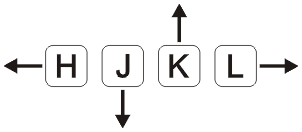
\includegraphics[width=5cm]{c7_vim_hjkl_02.png}
  \end{figure}
\end{frame}

\begin{frame}[fragile]
  \frametitle{移动和定位 | \alert{移动定位}}
  \begin{table}
    \centering
    \rowcolors[]{1}{blue!20}{blue!10}
    \begin{tabularx}{0.9\textwidth}{clX}
      \hline
      \rowcolor{blue!50}命令 & 说明 & 结果\\
      \hline
      0 & 零 & 光标移至行首\\
      \verb|^| & --- & 光标移至行首(第一个非空字符)\\
      \verb|$| & 美元符号 & 光标移至行尾\\
      \hline
      b & 小写b & 光标移至当前单词或前一个单词的开头\\
      B & 大写B & 同b,但不计算标点符号\\
      w & 小写w & 光标移至下一个单词的开头\\
      W & 大写W & 同w,但不计算标点符号\\
      e & 小写e & 光标移至当前单词或下一个单词的末尾\\
      E & 大写E & 同e,但不计算标点符号\\
      ge & --- & 光标移至上一个单词的末尾\\
      gE & --- & 同ge,但不计算标点符号\\
      \hline
    \end{tabularx}
  \end{table}
\end{frame}

\begin{frame}[fragile]
  \frametitle{移动和定位 | \alert{移动定位}}
  \begin{table}
    \centering
    \rowcolors[]{1}{blue!20}{blue!10}
    \begin{tabularx}{\textwidth}{clX}
      \hline
      \rowcolor{blue!50}命令 & 说明 & 结果\\
      \hline
      \verb=|= & 管道符 & 光标移至行首\\
      \verb=n|= & --- & 光标移至当前行的第n列\\
      \verb|_| & 下划线 & 光标移至行首\small{(第一个非空字符,支持向下计数)}\\
      \hline
      \verb|+| & 加号 & 光标移至下一行行首\\
      \verb|-| & 减号 & 光标移至上一行行首\\
      \hline
      gg & 两个小写g & 光标移至第一行(\verb|:0|)\\
      G & 大写G & 光标移至最后一行(\verb|:$|)\\
      xG & G前加数字 & 光标移至指定行\\
      \verb|:x| & 冒号后跟数字 & 光标移至指定行\\
      \hline
      \verb|(| & 左圆括号 & 光标移至当前句子或上一句子的开始处\\
      \verb|)| & 右圆括号 & 光标移至下一句子的开始处\\
      \hline
      \{ & 左大括号 & 光标移至段落的开始处\\
      \} & 右大括号 & 光标移至段落的结尾处\\
      \hline
    \end{tabularx}
  \end{table}
\end{frame}

\begin{frame}[fragile]
  \frametitle{移动和定位 | \alert{移动定位}}
  \begin{table}
    \centering
    \rowcolors[]{1}{blue!20}{blue!10}
    \begin{tabularx}{0.8\textwidth}{clX}
      \hline
      \rowcolor{blue!50}命令 & 说明 & 结果\\
      \hline
      \verb|*| & 星字符 & 向下查找光标下的单词\\
      \verb|#| & 井字符 & 向上查找光标下的单词\\
      \hline
      \% & 大中小括号 & 查找与光标下括号相配对的括号\\
      \hline
      fx & 向下查找 & 光标移至下一个x上\\
      Fx & 向上查找 & 光标移至上一个x上\\
      ; & 分号 & 同向查找\\
      , & 逗号 & 反向查找\\
      \hline
      tx & --- & 光标移至下一个x之前\\
      Tx & --- & 光标移至上一个x之后\\
      \hline
    \end{tabularx}
  \end{table}
\end{frame}

\begin{frame}[fragile]
  \frametitle{移动和定位 | 移动定位}
  \begin{table}
    \centering
    \rowcolors[]{1}{blue!20}{blue!10}
    \begin{tabularx}{\textwidth}{clX}
      \hline
      \rowcolor{blue!50}命令 & 说明 & 结果\\
      \hline
      \verb|''| & 两个单引号 & 光标移至上一个编辑位置\small{(所在行首个非空白字符)}\\
      \verb|'.| & 单引号加点号 & 同 \verb|''|\\
      \verb|``| & 两个反引号 & 光标移至上一个编辑位置\small{(精确到列)}\\
      \verb|`.| & 反引号加点号 & 同 \verb|``|\\
      \hline
      Ctrl+O & --- & 光标跳转至更老的编辑位置\\
      Ctrl+I & --- & 光标跳转至更新的编辑位置\\
      \hline
      mx & --- & 设置名为x的标记(mark)\\
      \verb|'x| & --- & 光标跳转至标记x\small{(所在行首个非空白字符)}\\
      \verb|`x| & --- & 光标跳转至标记x\small{(精确到列)}\\
      \hline
    \end{tabularx}
  \end{table}
\end{frame}

\begin{frame}[fragile]
  \frametitle{移动和定位 | 移动定位}
  \begin{table}
    \centering
    \rowcolors[]{1}{blue!20}{blue!10}
    \begin{tabularx}{0.9\textwidth}{clX}
      \hline
      \rowcolor{blue!50}命令 & 说明 & 结果\\
      \hline
      H & 大写H & 光标移至屏幕上端\\
      M & 大写M & 光标移至屏幕中央\\
      L & 大写L & 光标移至屏幕下端\\
      \hline
      zt & --- & 把光标所在行置于屏幕顶部\\
      zz & --- & 把光标所在行置于屏幕中部\\
      zb & --- & 把光标所在行置于屏幕底部\\
      \hline
      Ctrl+E & 同时按下Ctrl和E键 & 屏幕上滚\\
      Ctrl+Y & 同时按下Ctrl和Y键 & 屏幕下滚\\
      \hline
      Ctrl+F & 同时按下Ctrl和F键 & 向下滚动一屏\\
      Ctrl+B & 同时按下Ctrl和B键 & 向上滚动一屏\\
      Ctrl+D & 同时按下Ctrl和D键 & 向下滚动半屏\\
      Ctrl+U & 同时按下Ctrl和U键 & 向上滚动半屏\\
      \hline
      Ctrl+G & 同时按下Ctrl和G键 & 显示状态,确定光标位置\\
      \hline
    \end{tabularx}
  \end{table}
\end{frame}

\begin{frame}[fragile]
  \frametitle{移动和定位 | 移动定位 | 说明}
  \begin{table}
    \centering
    \rowcolors[]{1}{blue!20}{blue!10}
    \begin{tabularx}{\textwidth}{clX}
      \hline
      \rowcolor{blue!50}命令 & 说明 & 结果\\
      \hline
      \verb|:set nu| & 末行模式 & 显示行号\\
      \verb|:set nonu| & 末行模式 & 隐藏行号\\
      \verb|:set ic| & 末行模式(ignorecase) & 查找时忽略字母大小写\\
      \verb|:set is| & 末行模式(incsearch) & 查找短语时显示部分匹配\\
      \verb|:set hls| & 末行模式(hlsearch) & 高亮显示所有的匹配短语\\
      \hline
      --- & 单词 & 一组由空格、Tab或标点符号分隔开的字符\\
      --- & 句子 & 由后面跟两个空格的标点符号标识\\
      \hline
    \end{tabularx}
  \end{table}
\end{frame}

\section{编辑文件}
\subsection{进入输入模式}
\begin{frame}
  \frametitle{编辑 | \alert{进入输入模式}}
  \begin{table}
    \centering
    \rowcolors[]{1}{blue!20}{blue!10}
    \begin{tabularx}{0.9\textwidth}{clX}
      \hline
      \rowcolor{blue!50}命令 & 说明 & 结果\\
      \hline
      i & 小写i & insert,在光标前插入\\
      I & 大写I & 在行首处插入\\
      a & 小写a & append,在光标后插入\\
      A & 大写A & 在行尾处插入\\
      o & 小写o & 在光标所在行的下面插入新行\\
      O & 大写O & 在光标所在行的上面插入新行\\
      \hline
      2O & 命令前加数字 & 在光标所在行的上面插入两个新行\\
      \hline
    \end{tabularx}
  \end{table}
\end{frame}

\subsection{剪切删除}
\begin{frame}[fragile]
  \frametitle{编辑 | \alert{剪切删除}}
  \begin{table}
    \centering
    \rowcolors[]{1}{blue!20}{blue!10}
    \begin{tabularx}{0.9\textwidth}{clX}
      \hline
      \rowcolor{blue!50}命令 & 说明 & 结果\\
      \hline
      x & 小写x & 删除光标所在位置的字符\\
      X & 大写X & 删除光标前的字符\\
      dw & 小写dw & 从光标处删除至下一个单词\\
      \verb|d^| & --- & 从光标前删除至行首\\
      \verb|d$| & --- & 从光标处删除至行尾\\
      dG & --- & 从光标所在行删除至最后一行\\
      D & 大写D & 从光标处删除至行尾\\
      dd & 小写dd & 删除光标所在行\\
      \hline
      3x & 命令前加数字 & 删除光标所在位置开始的后3个字符\\
      3dd, d3d & 命令前加数字 & 删除3行\\
      \verb|:m,nd| & --- & 从第m行删除到第n行\\
      \hline
      ddO & 组合命令 & 删除光标所在行并创建新行\\
      \hline
    \end{tabularx}
  \end{table}
\end{frame}

\begin{frame}[fragile]
  \frametitle{编辑 | \alert{剪切删除}}
  \begin{table}
    \centering
    \rowcolors[]{1}{blue!20}{blue!10}
    \begin{tabularx}{0.8\textwidth}{clX}
      \hline
      \rowcolor{blue!50}命令 & 说明 & 结果\\
      \hline
      \verb|di(| & --- & 删除引号、括号等内部的文字\\
      \verb|da(| & --- & 删除引号、括号等及其内部的文字\\
      \verb|dtx| & --- & 删除至x(删除x前的内容)\\
      \hline
    \end{tabularx}
  \end{table}
\end{frame}

\subsection{修改替换}
\begin{frame}
  \frametitle{编辑 | \alert{修改替换}}
  \begin{table}
    \centering
    \rowcolors[]{1}{blue!20}{blue!10}
    \begin{tabularx}{0.9\textwidth}{clX}
      \hline
      \rowcolor{blue!50}命令 & 说明 & 结果\\
      \hline
      cc & 两个小写c & 修改光标所在行\\
      cw & 小写cw & 修改光标所在的单词(光标处至单词结束),进入输入模式\\
      r & 小写r & 替换光标处的字符,替换后返回命令模式\\
      R & 大写R & 从光标处开始替换字符,直至按Esc停止\\
      s & 小写s & 替换光标处的字符,替换后处于输入模式\\
      S & 大写S & 替换光标所在行,替换后处于输入模式\\
      \hline
    \end{tabularx}
  \end{table}
\end{frame}

\subsection{复制粘贴}
\begin{frame}
  \frametitle{编辑 | \alert{复制粘贴}}
  \begin{table}
    \centering
    \rowcolors[]{1}{blue!20}{blue!10}
    \begin{tabularx}{0.9\textwidth}{clX}
      \hline
      \rowcolor{blue!50}命令 & 说明 & 结果\\
      \hline
      J & 大写J & 合并光标所在行和其下一行\\
      \hline
      yy & 两个小写y & 复制光标所在行\\
      Y & 大写Y & 复制光标所在行\\
      yw & 小写yw & 复制光标所在的单词(光标处至单词结尾)\\
      \hline
      p & 小写p & 在光标后粘贴\\
      P & 大写P & 在光标前粘贴\\
      \hline
      3yy, y3y & 命令前加数字 & 复制从光标所在行开始的3行内容\\
      \hline
    \end{tabularx}
  \end{table}
\end{frame}

\subsection{撤销重做}
\begin{frame}
  \frametitle{编辑 | \alert{撤销重做}}
  \begin{table}
    \centering
    \rowcolors[]{1}{blue!20}{blue!10}
    \begin{tabularx}{0.8\textwidth}{clX}
      \hline
      \rowcolor{blue!50}命令 & 说明 & 结果\\
      \hline
      u & 小写u & 撤销最近一次的编辑\\
      U & 大写U & 撤销光标所在行的所有编辑\\
      Ctrl+R & 同时按下Ctrl和R键 & 重做\\
      \hline
      \verb|.| & 句点 & 重复上一个命令\\
      \hline
    \end{tabularx}
  \end{table}
\end{frame}

\subsection{搜索替换}
\begin{frame}[fragile]
  \frametitle{编辑 | 搜索替换 | \alert{搜索}}
  \begin{table}
    \centering
    \rowcolors[]{1}{blue!20}{blue!10}
    \begin{tabularx}{0.6\textwidth}{cX}
      \hline
      \rowcolor{blue!50}命令 & 结果\\
      \hline
      \verb|/word| & 从光标处向下搜索word \\
      \verb|?word| & 从光标处向上搜索word\\
      n & 同向定位下一个搜索\\
      N & 反向定位下一个搜索\\
      \hline
    \end{tabularx}
  \end{table}
\end{frame}

\begin{frame}[fragile]
  \frametitle{编辑 | 搜索替换 | \alert{替换}}
  \begin{table}
    \centering
    \rowcolors[]{1}{blue!20}{blue!10}
    \begin{tabularx}{\textwidth}{cX}
      \hline
      \rowcolor{blue!50}命令 & 结果\\
      \hline
      \verb|:s/old/new/| & 将光标所在行上的第一个old替换为new\\
      \verb|:s/old/new/g| & globally,将光标所在行的所有old替换为new\\
      \verb|:s/old/new/c| & 替换时进行确认\\
      \verb|:m,ns/old/new/g| & 将从第m行到第n行的所有old替换为new\\
      \verb|:1,$s/old/new/g| & 将整个文件内的所有old替换为new\\
      \verb|:|\%\verb|s/old/new/g| & 将整个文件内的所有old替换为new\\
      \verb|:|\%\verb|s/\<old\>/new/g| & 将整个文件内的所有old单词替换为new\\
      \hline
    \end{tabularx}
  \end{table}
\end{frame}

\begin{frame}[fragile]
  \frametitle{编辑 | 搜索替换 | \alert{替换}}
  \begin{table}
    \centering
    \rowcolors[]{1}{blue!20}{blue!10}
    \begin{tabularx}{0.9\textwidth}{cX}
      \hline
      \rowcolor{blue!50}命令 & 结果\\
      \hline
      默认 & 对光标所在行进行操作\\
      \verb|m,n| & 在从第m行到第n行范围内进行操作\\
      \% & 在整个文件内进行操作\\
      \verb|/g| & globally,对所有匹配进行替换\\
      \verb|/c| & 每次替换前进行询问确认\\
      \hline
      \verb|:m,ns/^/#/g| & 进行连续行注释\\
      \verb|:m,ns/^#//g| & 删除连续行注释\\
      \hline
      \verb|&| & 重复最后一个替换命令(\verb|:s|)\\
      \hline
    \end{tabularx}
  \end{table}
\end{frame}

\subsection{保存退出}
\begin{frame}
  \frametitle{\alert{保存退出}}
  \begin{table}
    \centering
    \rowcolors[]{1}{blue!20}{blue!10}
    \begin{tabularx}{\textwidth}{cX}
      \hline
      \rowcolor{blue!50}命令 & 结果\\
      \hline
      \verb|:q| & 未修改,退出Vim编辑器\\
      \verb|:w| & 写入修改,保存当前文件\\
      \verb|:w filename| & 文件另存为filename\\
      \verb|:wq| & 保存文件并退出\\
      \verb|ZZ| & 同 \verb|:wq|\\
      \verb|:x| & 保存文件并退出\\
      \hline
      \verb|:q!| & 放弃对文件的修改并退出\\
      \verb|:w! filename| & 覆盖文件\\
      \verb|:wq!| & 保存修改并退出(文件所有者可忽略文件的只读属性)\\
      \hline
      \verb|:e!| & 打开文件的上一次成功写入的版本\\
      \verb|:r /path/filename| & 插入filename文件的内容\\
      \hline
    \end{tabularx}
  \end{table}
\end{frame}

\subsection{命令补遗}
\begin{frame}[fragile]
  \frametitle{命令补遗}
  \begin{table}
    \centering
    \rowcolors[]{1}{blue!20}{blue!10}
    \begin{tabularx}{0.7\textwidth}{cX}
      \hline
      \rowcolor{blue!50}命令 & 结果\\
      \hline
      v & 进入可视模式\\
      V & 进入行可视模式\\
      Ctrl+V & 进入块/列可视模式\\
      \hline
      \verb|~| & 转换光标下字符的大小写\\
      \hline
      \verb|>| & 可视模式,缩进\\
      \verb|>>| & 行首缩进\\
      \verb|<| & 可视模式,反向缩进\\
      \verb|<<| & 行首反向缩进\\
      \verb|=| & 可视模式,自动缩进/格式化\\
      \verb|==| & 自动缩进\\
      \hline
      qx & 录制宏,命名为x,按q键结束录制\\
      \verb|@x| & 运行名为x的宏\\
      \hline
      K & 查找光标下单词的man page\\
      \hline
    \end{tabularx}
  \end{table}
\end{frame}

\begin{frame}[fragile]
  \frametitle{命令补遗}
  \begin{table}
    \centering
    \rowcolors[]{1}{blue!20}{blue!10}
    \begin{tabularx}{0.8\textwidth}{cX}
      \hline
      \rowcolor{blue!50}命令 & 结果\\
      \hline
      \verb|:split| & 横向分割窗口\\
      \verb|:vsplit| & 纵向分割窗口\\
      \verb|:diffsplit| & 以横向比较模式分割窗口\\
      \verb|:vert diffsplit| & 以纵向比较模式分割窗口\\
      Ctrl+W Ctrl+W & 在窗口间跳转\\
      Ctrl+W p & 在窗口间跳转(下一个窗口)\\
      Ctrl+W h/j/k/l & 在窗口间跳转\\
      \hline
    \end{tabularx}
  \end{table}
\end{frame}

\begin{frame}[fragile]
  \frametitle{命令补遗}
  \begin{table}
    \centering
    \rowcolors[]{1}{blue!20}{blue!10}
    \begin{tabularx}{\textwidth}{cX}
      \hline
      \rowcolor{blue!50}命令 & 结果\\
      \hline
      缩写 & \verb|:ab asap as soon as possible|\\
      \hline
      \verb|:w !sudo tee| \% & 忘记用root打开文件时的文件保存\\
      \hline
      \verb|:earlier 1m| & 按时间回退文件\\ 
      \verb|:later| & 与上述相反\\ 
      \hline
      基本计算器 & 插入模式下,依次:Ctrl+R,=,算式,Enter\\
      \hline
      \verb|:TOhtml| & 把当前文件转换成网页\\
      \hline
      \verb|:help| & 打开帮助窗口\\
      \verb|:help CMD| & 找到关于CMD命令的帮助信息\\
      \hline
      Ctrl+N & 输入模式,自动补全\\
      \hline
      Ctrl+D & 输入 \verb|:|命令时,查看可能的补全结果\\
      Tab & 输入 \verb|:|命令时自动补全\\
      \hline
      vimdiff & 比较两个文件的不同(在终端中使用)\\
      \verb|~/.vimrc| & 使用vimrc启动脚本文件保存用户偏好设置\\
      \hline
      更多 & 等待你去发现\\
      \hline
    \end{tabularx}
  \end{table}
\end{frame}

\section{Vim进阶}
\subsection{运行命令}
\begin{frame}[fragile]
  \frametitle{进阶 | \alert{运行命令}}
  \begin{table}
    \centering
    \rowcolors[]{1}{blue!20}{blue!10}
    \begin{tabularx}{\textwidth}{cX}
      \hline
      \rowcolor{blue!50}命令 & 结果\\
      \hline
      \verb|:!command| & 在Vim中运行命令,按任意键返回Vim\\
      \verb|:!ls| & 在Vim中运行ls命令\\
      \hline
      \verb|:!wc| \% & 在Vim中运行wc命令(\%代表当前文件)\\
      \hline
      \verb|:r !command| & 插入命令执行结果\\
      \verb|:r !date| & 插入日期和时间\\
      \verb|:r !sed -n 1,3p filename| & 插入fielname文件的1-3行内容\\
      \hline
    \end{tabularx}
  \end{table}
\end{frame}

\subsection{Vim插件}
\begin{frame}
  \frametitle{进阶 | Vim插件}
  \begin{figure}
    \centering
    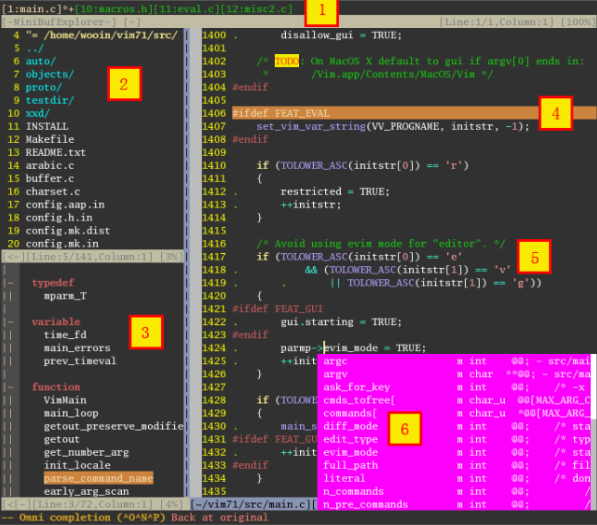
\includegraphics[width=12cm,height=8cm]{c7_vim_plugin_01.png}
  \end{figure}
\end{frame}

\section{Vim命令集锦}
\begin{frame}
  \frametitle{Vim命令集锦 | 命令组合}
  \begin{figure}
    \centering
    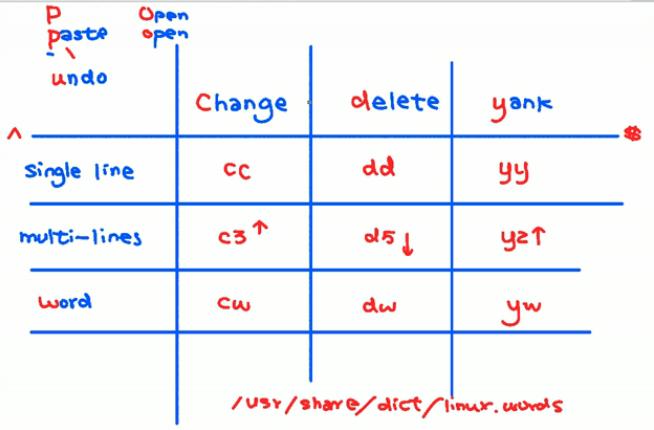
\includegraphics[width=10cm]{c7_vim_command_01.png}
  \end{figure}
\end{frame}

\begin{frame}
  \frametitle{Vim命令集锦}
  \begin{figure}
    \centering
    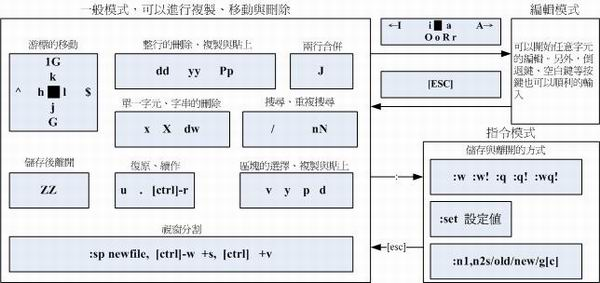
\includegraphics[width=11cm]{c7_vim_command_02.jpg}
  \end{figure}
\end{frame}

\begin{frame}
  \frametitle{Vim命令集锦}
  \begin{figure}
    \centering
    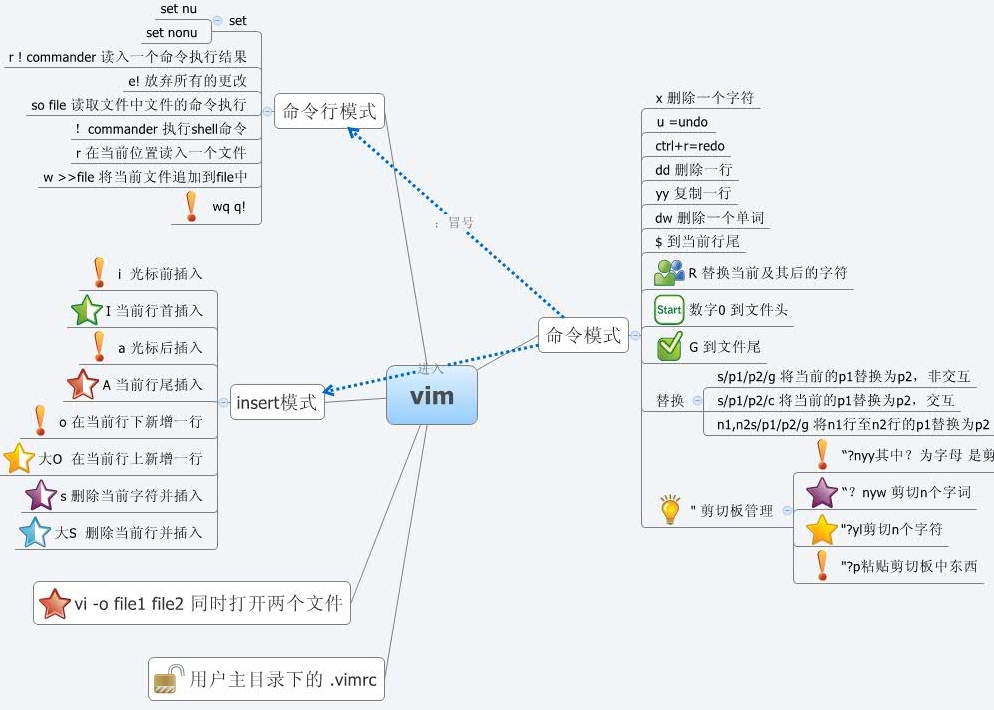
\includegraphics[width=12cm]{c7_vim_shortcut_01.jpg}
  \end{figure}
\end{frame}

\begin{frame}
  \frametitle{Vim命令集锦}
  \begin{figure}
    \centering
    
\includegraphics[width=12cm,height=8cm]{c7_vim_shortcut_02.jpg}
  \end{figure}
\end{frame}

\begin{frame}
  \frametitle{Vim命令集锦}
  \begin{figure}
    \centering
    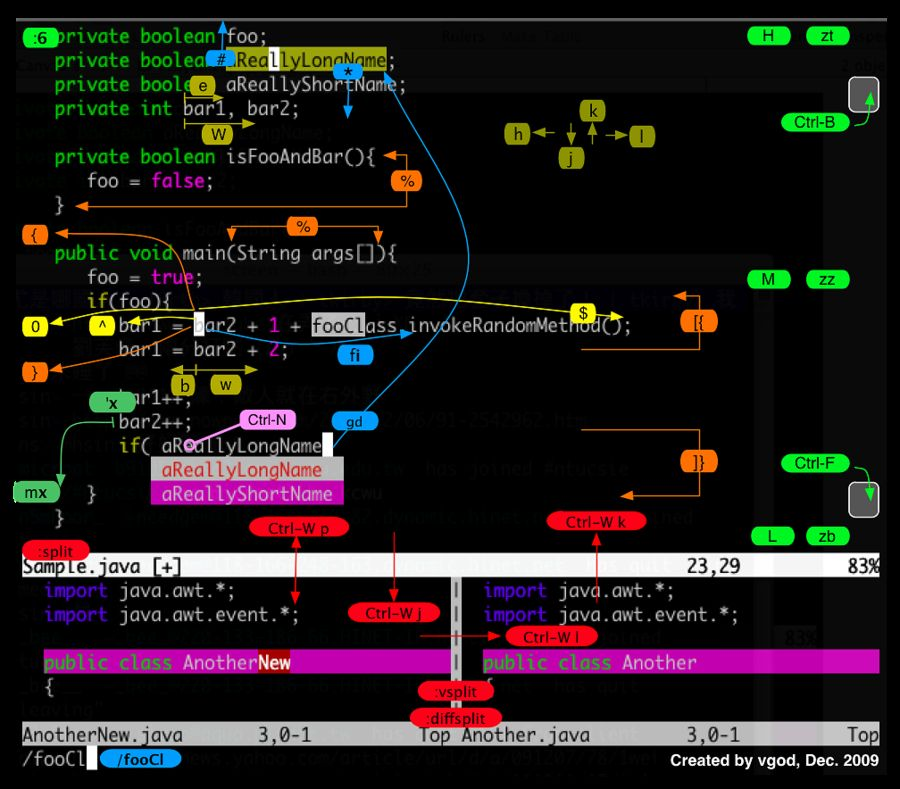
\includegraphics[width=12cm,height=8cm]{c7_vim_shortcut_03.jpg}
  \end{figure}
\end{frame}

\begin{frame}
  \frametitle{Vim命令集锦}
  \begin{figure}
    \centering
    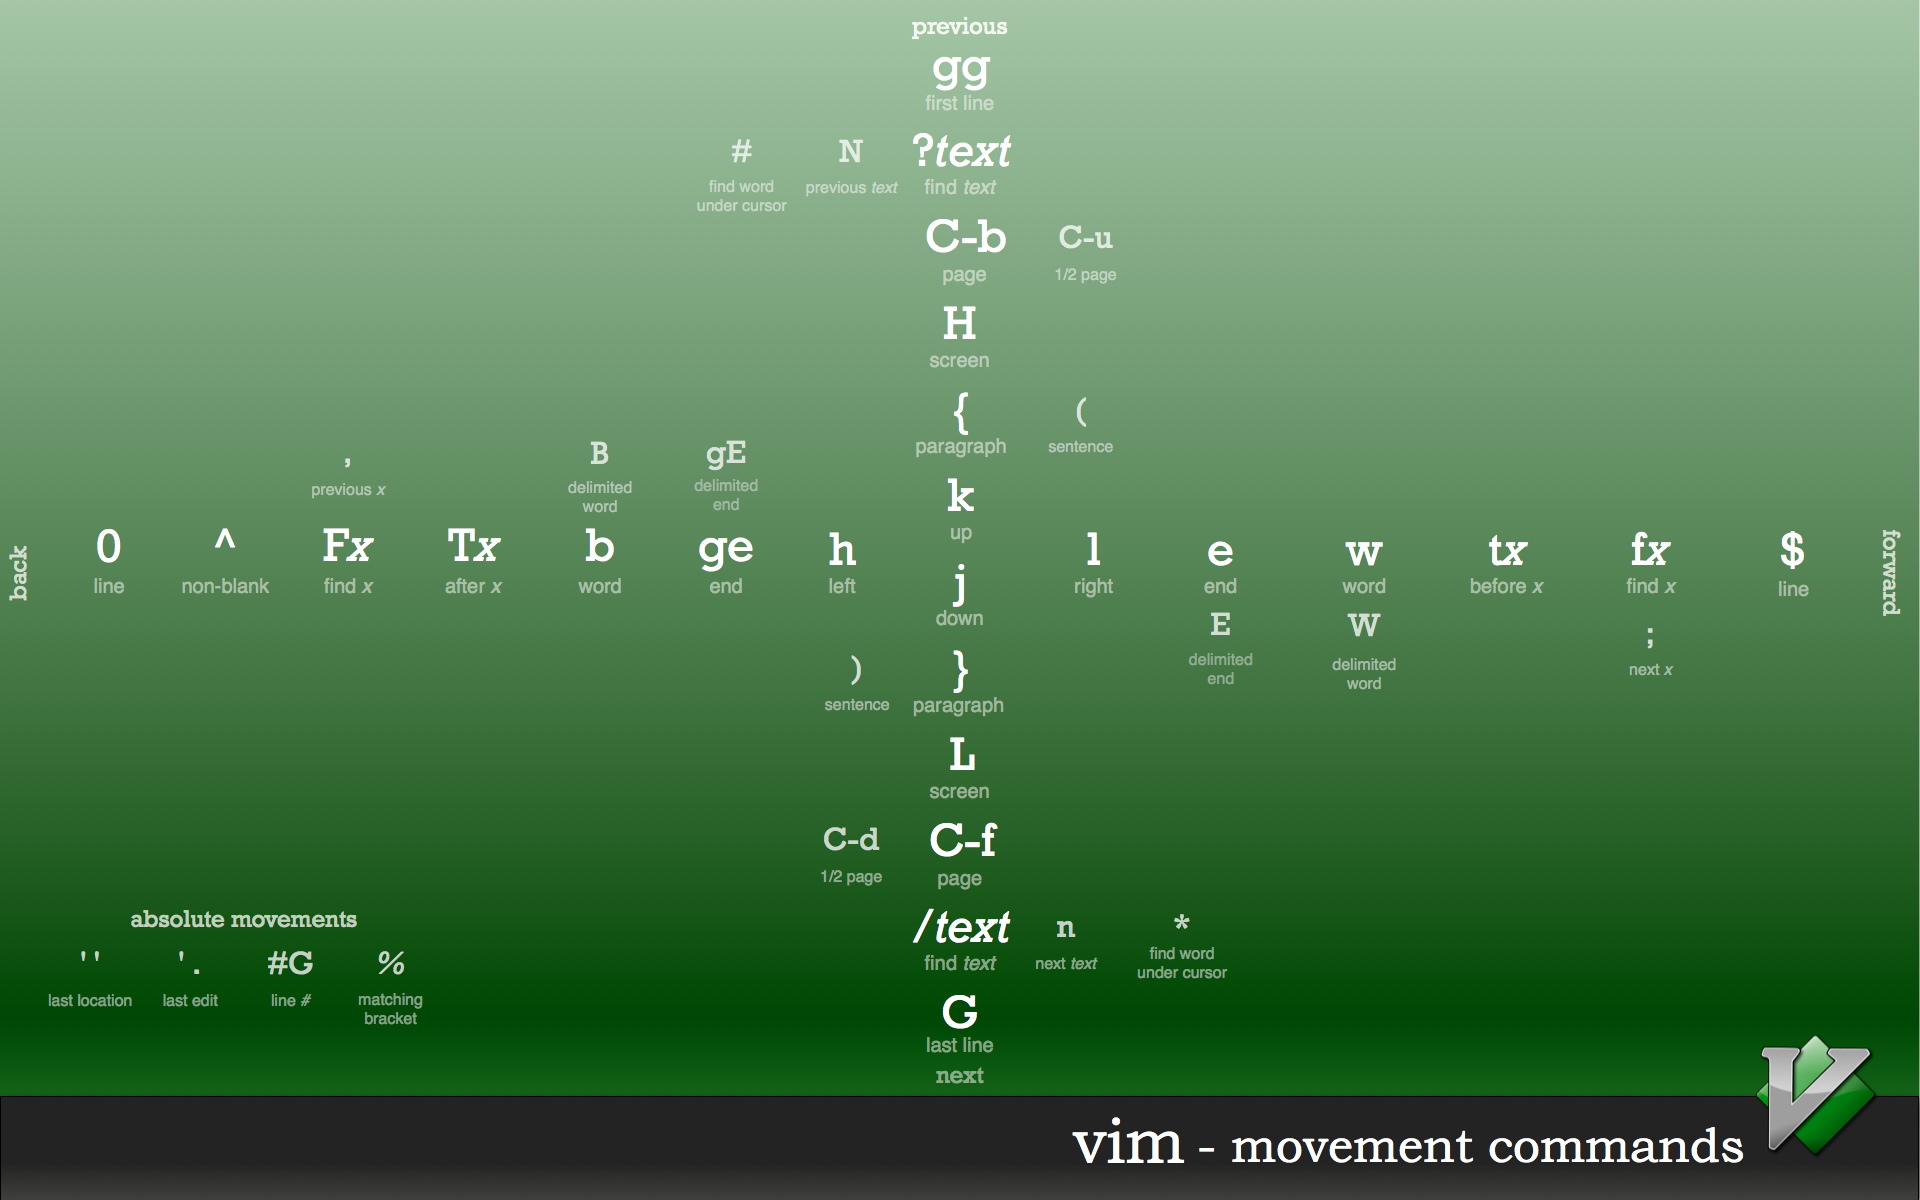
\includegraphics[width=12cm]{c7_vim_shortcut_04.png}
  \end{figure}
\end{frame}

\begin{frame}
  \frametitle{Vim命令集锦}
  \begin{figure}
    \centering
    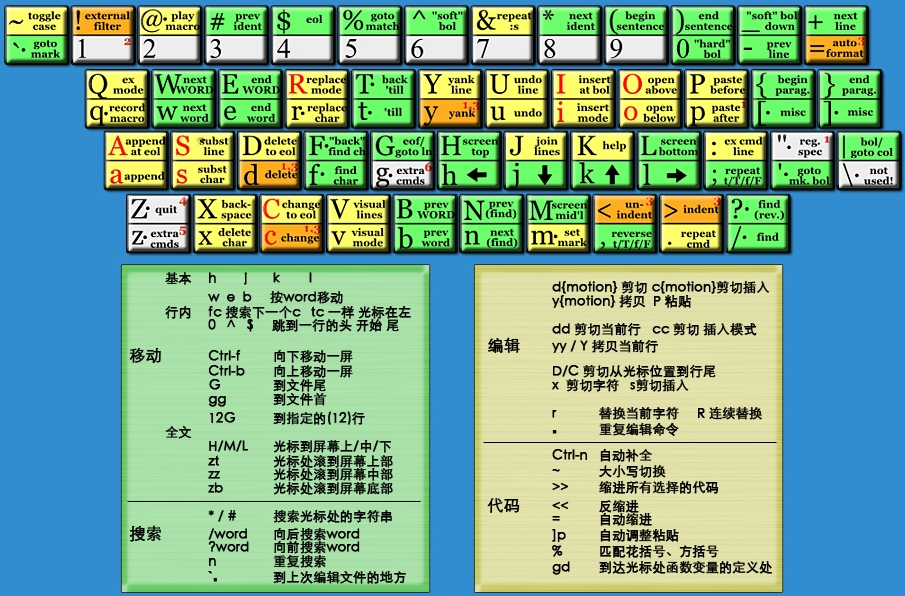
\includegraphics[width=12cm]{c7_vim_shortcut_05.jpg}
  \end{figure}
\end{frame}

\begin{frame}
  \frametitle{Vim命令集锦}
  \begin{figure}
    \centering
    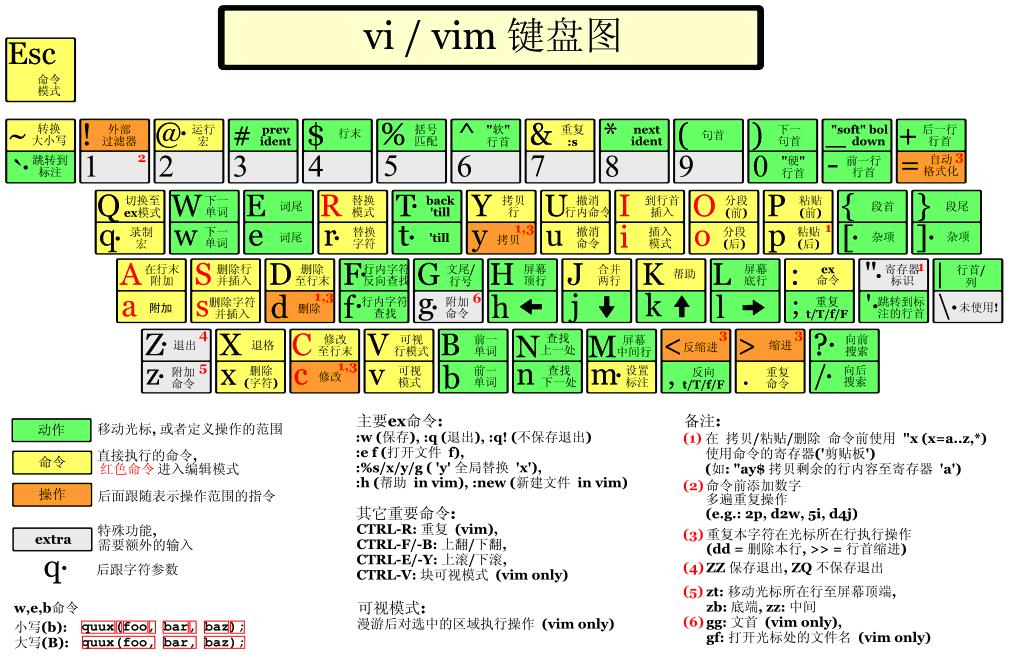
\includegraphics[width=12cm]{c7_vim_shortcut_06.jpg}
  \end{figure}
\end{frame}

\begin{frame}
  \frametitle{Vim命令集锦 | 键盘布局}
  \begin{figure}
    \centering
    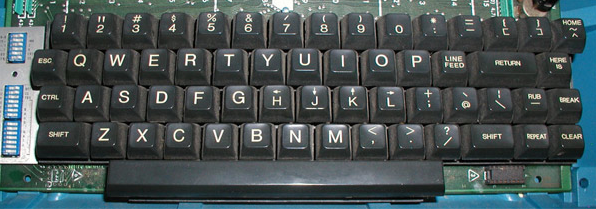
\includegraphics[width=12cm]{c7_vim_keyboard.png}
  \end{figure}
\end{frame}

\section{Vim语言}
\begin{frame}
  \frametitle{Vim语言 | 词汇 | 简介}
  \begin{block}{动词}
    动词代表了我们打算对文本进行什么样的操作。
  \end{block}
  \pause
  \begin{block}{名词}
    名词代表了我们即将处理的文本对象(text object)。
  \end{block}
  \pause
  \begin{block}{介词}
    介词界定了待编辑文本的范围或者位置。
  \end{block}
\end{frame}

\begin{frame}
  \frametitle{Vim语言 | 词汇}
  \begin{columns}
    \column{0.32\textwidth}
  \begin{block}{动词}
    \begin{itemize}
      \item d:delete,删除
      \item r:replace,替换
      \item c:change,修改
      \item y:yank,复制
      \item v:visual select,选取
    \end{itemize}
  \end{block}
  \pause
    \column{0.35\textwidth}
   \begin{block}{名词}
    \begin{itemize}
      \item w:word,单词
      \item s:sentence,句子
      \item p:paragraph,段落
      \item t:tag,HTML标签
    \end{itemize}
   \end{block}
  \pause
    \column{0.25\textwidth}
  \begin{block}{介词}
    \begin{itemize}
      \item i:inside,在…之内
      \item a:around,环绕…
      \item t:to,到…位置前
      \item f:forward,到…位置上
    \end{itemize}
  \end{block}
 \end{columns}
\end{frame}

\begin{frame}
  \frametitle{Vim语言 | 造句}
  \begin{block}{基本语法}
  动词 + 介词 + 名词
  \end{block}
  \pause
  \begin{block}{实例}
    \begin{itemize}
      \item dip:delete inside paragraph,删除一个段落
      \item vis:visual select inside sentence,选区一个句子
      \item ciw:change inside word,修改一个单词
      \item caw:change around word,修改一个单词
      \item dtx:delete to x,删除文本直到字符“x”前(不包括字符“x”)
      \item dfx:delete forward x,删除文本直到字符“x”上(包括字符“x”)
    \end{itemize}
  \end{block}
\end{frame}

\begin{frame}
  \frametitle{Vim语言 | 词汇 | 补充}
  \begin{block}{数词}
    数词指定了待编辑文本对象的数量,从这个角度而言,数词也可以看作是一种介词。
  \end{block}
  \pause
  \begin{block}{造句语法}
  动词 + 介词/数词 + 名词
  \end{block}
  \pause
  \begin{block}{实例}
    \begin{itemize}
      \item c3w:change three words,修改三个单词
      \item d2w:delete two words,删除两个单词
    \end{itemize}
  \end{block}
\end{frame}

\begin{frame}
  \frametitle{Vim语言 | 词汇 | 补充}
  \begin{block}{补充}
    数词也可以修饰动词,表示将操作执行n次。
  \end{block}
  \pause
  \begin{block}{对应语法}
  数词 + 动词 + 名词
  \end{block}
  \pause
  \begin{block}{实例}
    \begin{itemize}
      \item 2dw:twice delete word,两次删除单词(等价于删除两个单词)
      \item 3x:three times delete character,三次删除字符(等价于删除三个字符)
    \end{itemize}
  \end{block}
\end{frame}

\section{回顾与总结}
\subsection{总结}
\begin{frame}
  \frametitle{Vim | 总结}
  \begin{block}{知识点}
    \begin{itemize}
      \item Vim的主要工作模式:命令模式、输入模式、末行模式
      \item Vim的启动和退出:启动,保存,退出
      \item Vim中的移动和定位
      \item Vim中的文本编辑:进入输入模式,修改删除、复制粘贴、搜索替换
      \item 在Vim中运行系统命令
      \item Vim的学习:用户手册,帮助系统,命令总结
    \end{itemize}
  \end{block}
  \begin{block}{技能}
    \begin{itemize}
      \item 使用Vim进行日常的文本编辑
    \end{itemize}
  \end{block}
\end{frame}

\subsection{思考题}
\begin{frame}
  \frametitle{Vim | 思考题}
  \begin{enumerate}
    \item Vim的工作模式主要有哪三种?
    \item 在Vim中如何进行模式的转换?
    \item Vim中最基本的移动命令是哪四个?
    \item 进入Vim输入模式的命令有哪些?
    \item 在Vim中如何进行剪切、复制和粘贴?
    \item 在Vim中如何进行撤销和重做?
    \item 在Vim中如何进行搜索和替换?
    \item 在Vim中如何运行系统命令?
    \item 启动、保存文件和退出Vim的命令有哪些?
  \end{enumerate}
\end{frame}

\begin{frame}
  \frametitle{下节预告}
  还记得学习过的C语言吗?试着编写几个小程序,读取输入、条件判断、循环迭代、编写函数、……
\end{frame}



\section*{Acknowledgements}
\begin{frame}
  \frametitle{Powered by}
  \begin{center}
    
\includegraphics[width=9cm]{power.png}
  \end{center}
\end{frame}

\end{document}


